%%%%%%%%%%%%%%%%%%%%%%%%%%%%%%%%%%%%%%%%%%%%%%%%%%%%%%%%%%%%%%%%%%%%%%%%
%                                                                      %
%     File: Thesis_Results.tex                                         %
%     Tex Master: Thesis.tex                                           %
%                                                                      %
%     Author: Andre C. Marta                                           %
%     Last modified :  2 Jul 2015                                      %
%                                                                      %
%%%%%%%%%%%%%%%%%%%%%%%%%%%%%%%%%%%%%%%%%%%%%%%%%%%%%%%%%%%%%%%%%%%%%%%%

\chapter{Adding a new product when already producing one}
\label{chapter:2}

Insert your chapter material here...

%%%%%%%%%%%%%%%%%%%%%%%%%%%%%%%%%%%%%%%%%%%%%%%%%%%%%%%%%%%%%%%%%%%%%%%%
\section{Introduction}
\label{section:2_intro}

Situação do problema.
Trabalhos já realizados e de maneira os extendemos.

Some overview of the underlying theory about the topic...


%%%%%%%%%%%%%%%%%%%%%%%%%%%%%%%%%%%%%%%%%%%%%%%%%%%%%%%%%%%%%%%%%%%%%%%%
\section{Stopping Problem}
\label{section:2_theory}



\subsection{Benchmark Model}
\label{subsec:2_bm}

\subsection{Capacity Optimization Model}
\label{subsec:2_com}



\section{Maximization Problem}


\section{Comparative Statics}
Since the obtained results cannot reduce to each other, we will treat each case separately, starting with the simplest one derived in \ref{subsec:2_bm}.

\subsection{Benchmark Model}
In this section we study the behaviour of the decision threshold $x^*_B$ and $x^*_{C}$ and $K^*$ as described in \eqref{label}, with
the different parameters.

Comparisons between the benchmark and capacity optimization models will be made.\\
\textbf{Proposition:}
Decision threshold $x^*_B$ increases with $ \delta, \ \sigma$ and $\alpha$ only when $\theta > \frac{K_1}{ K_0^2} (K_0+K_1 r \delta)$, decreases with $\theta$ and $\alpha$ only when $\theta < \frac{K_1}{ K_0^2} (K_0+K_1 r \delta)$ and does not have a monotonic behaviour with $K_0, \ K_1, \ \mu, \ r$.


\textbf{Proof:}

Regarding the formula obtained for  $x^*_B$, we immediately conclude that the decision threshold increases with $\delta$ and decreases with $\theta$.

Regarding $\sigma$, we observe that


$$    \frac{\partial x^*_B ( \sigma ) }{\partial \sigma}= 
\frac{(r-\mu )  \left(\delta  K_1+\frac{K_0(1-\alpha K_0)}{r}\right)}{(d_1-1) K_1 (\theta -\alpha  K_1)} \left(\frac{2 \mu }{\sigma ^3}+\frac{\frac{4 \mu  \left(\frac{1}{2}-\frac{\mu }{\sigma ^2}\right)}{\sigma ^3}-\frac{4 r}{\sigma ^3}}{2 \sqrt{\left(\frac{1}{2}-\frac{\mu }{\sigma ^2}\right)^2+\frac{2 r}{\sigma ^2}}}\right) \left( 1- \frac{d_1}{(d_1-1)^2} \right).$$


Taking into account our initial assumptions about $r, \ \mu$ and profits associated to the old and the new product, it follows that the leftmost expression is always positive. Since $d_1^2-d_1+1>0 \ \ \forall d_1$, the rightmost expression is also positive. Now we need to analyse the expression in between. We chec

Problemas em mostrar quando é que a segunda derivada é positiva.

Regarding $K_0$, we observe that

\begin{align*}
    \frac{\partial x^*_B ( K_0 ) }{\partial K_0}= 
\frac{d_1 (r-\mu )}{r (d_1-1)K_1(\theta-\alpha K_1)} (1-2\alpha K_0)
=
\begin{cases}
>0 &\ \text{for} \ K_0<\frac{1}{2 \alpha}\\
<0 &\ \text{for} \ K_0>\frac{1}{2 \alpha}
\end{cases}.
\end{align*}
since the expression represented in fraction is always positive.


Regarding $K_1$, we obtain that

\begin{align*}
\frac{\partial x^*_B ( K_1 ) }{\partial K_1}= 
\frac{d_1 (r-\mu )}{ (d_1-1)K_1(\theta-\alpha K_1)}  \left( \frac{\alpha (\frac{K_0(1-\alpha K_0)}{r}+K_1 \delta )}{\theta-\alpha K_1} -\frac{ \frac{K_0(1-\alpha K_0)}{r}+K_1 \delta )}{K_1}+ \delta \right)
\end{align*}


The leftmost expression is always positive. Thus we only need to evaluate the sign of the expression next to it. Manipulating mentioned expression, taking into account that the capacity level cannot be negative as well as the price function given by $\pi_0=K_0(1-\alpha K_0)$, it follows that

\begin{align*}
\frac{\partial x^*_B ( K_1 ) }{\partial K_1}= 
\begin{cases}
>0 &\ \text{for} \ K_1>\frac{-\pi_0+\sqrt{\alpha \pi_0 (\pi_0 + r \delta \theta)}}{ r\alpha \delta}\\
<0 &\ \text{for} \ K_1 \in \left[ 0, \frac{-\pi_0+\sqrt{\alpha \pi_0(\pi_0 + r \delta \theta)}}{ r\alpha \delta} \right]
\end{cases},
\end{align*}
from which we obtain that $x^*_B$ has no monotonic behaviour with $K_1$.


Regarding parameter $\alpha$, we obtain that

\begin{align*}
\frac{\partial x^*_B ( \alpha ) }{\partial \alpha}= 
\frac{d_1 (r-\mu )}{ (d_1-1)(\theta-\alpha K_1)}  \left( \frac{\frac{K_0(1-\alpha K_0)}{r}+ \delta K_1  }{\theta-\alpha K_1} -\frac{ K_0^2}{r K_1} \right),
\end{align*}
where the leftmost expression is always positive. Simplifying the expression in the biggest brackets to the same denominator, we obtain that
\begin{align*}
\frac{\partial x^*_B ( \alpha ) }{\partial \alpha}= 
\begin{cases}
>0 &\ \text{for} \ \theta < \frac{K_0 K_1 +K_1^2 r\delta}{K_0^2}\\
<0 &\ \text{for} \ \theta > \frac{K_0 K_1 +K_1^2 r\delta}{K_0^2}.
\end{cases}
\end{align*}

Note that the sign of the partial derivative does not depend on $\alpha$.

Regarding parameters $\mu$ and $r$ we obtained complex derivates, from which we weren't able to deduce any analytical results. However, as it will be showed right after this proof, using Mathematica we obtained that $x^*_B$ behaves in a non-monotonic way with $\mu$ and $r$.

\begin{flushright}
	$\square$
\end{flushright}




\subsection{Capacity Optimization Model}

\textbf{Proposition:}
Decision threshold $x^*_C$ increase with $K_0, \ \alpha, \ \delta$, decreases asymptotically with $\theta$ and do not have a monotonic behaviour with $\mu, \ r$.


\textbf{Proof:}

For the sake of simplicity, we will denote, in this proof, 
$\phi:=\sqrt{\frac{4 \mu ^2}{\sigma ^4}-\frac{4 \mu }{\sigma ^2}+\frac{8 r}{\sigma ^2}+1}>0$ and
$\psi:=4 d_1^2 \pi_0  (\delta  \theta  r+\pi_0 )+\delta ^2 \theta ^2 r^2>0$.
Recall also that $\pi_0>0$ stands for the profit function associated to the new product.

Regarding the formula obtained for  $x^*_C$, we immediately obtain that the decision threshold increases with $K_0$ and $\alpha$.


Regarding $\delta$, we obtain that

\begin{align*}
\frac{\partial x^*_B ( \delta ) }{\partial \delta}= \frac{(r-\mu ) \left(\frac{4 d_1^2 \theta  r \pi_0 +2 \delta  \theta ^2 r^2}{2 \sqrt{\psi }}+d_1 \theta  r\right)}{(d_1-1) \theta ^2 r}>0
\end{align*}
from which the result holds.

Regarding $\theta$, we obtain that

\begin{align*}
\frac{\partial x^*_B ( \theta) }{\partial \theta}= \frac{ \theta (r-\mu ) \left(\frac{4 \delta  d_1^2 r \omega +2 \delta ^2 \theta  r^2}{2 \sqrt{\psi }}+\delta  d_1 r\right)- 2 (r-\mu ) \left(d_1 (\delta  \theta  r+2 \omega )+\sqrt{\psi }\right)}{(d_1-1) \theta ^3 r}.
\end{align*}

Manipulating the numerator, it simplifies to
$$
\frac{\delta  d_1 r \left(2 d_1 (1-4 \theta ) \omega +(1-2 \theta ) \sqrt{\psi }\right)-4 d_1 \omega  \left(2 d_1 \omega +\sqrt{\psi }\right)+\delta ^2 \theta ^2 \left(-r^2\right)}{\sqrt{\psi}}$$
which is always negative for innovation levels $\theta>1/2$. COMPLETAR: ARRANJAR SUPOSIÇÃO MAIS FORTE

Since we assume that innovation levels have no upper limit, we evaluated them asymptotically. Denoting $\theta_A:=\frac{(r-\mu )}{(d_1-1) r}  \left(\sqrt{\delta ^2 r^2}+\frac{\delta  r \left(\sigma ^2 (\phi +1)-2 \mu \right)}{2 \sigma ^2}\right)>0$ we obtain that $x^*_C$ decreases on order of $\frac{\theta_A}{\theta}$, that is,  

$$x^*_C(\theta) \sim \frac{\theta_A}{\theta} \ \Leftrightarrow \ \lim_{\theta \to \infty} \frac{x^*_C(\theta)}{\frac{\theta_A}{\theta}}=1.$$

Regarding parameters $\mu$ and $r$, we obtain complex derivates, from which we couldn't deduce any analytical result. However, as it will be showed hereunder, $x^*_C$ behaves in a non-monotonic way with both $\mu$ and $r$.
\begin{flushright}
	$\square$
\end{flushright}


Although we couldn't obtain any analytical (strong) evidence, after different experiments done using \textit{Mathematica} and its function \texttt{Manipulate}, we obtained that decision thresholds $x^*_B$ and $x^*_C$ increase with volatility $\sigma$.



To illustrate results above mentioned we performed some numerical illustrations, using software \textit{Mathematica} and its function \texttt{Manipulate}. However here are only able to present static plots - we leave to the interested ones, to see the results achieved with \texttt{Manipulate}.

Unless it is written the opposite, following values were considered:
\begin{table*}[!htb]
	\centering
	%\label{my-label}
	\begin{tabular}{lllllll}
		$\bullet$ & $\mu=0.03$     &  & \hspace{7cm} &  &  $\bullet$ & $\alpha=0.01$ \\
		$\bullet$ & $\sigma=0.005$ &  & \hspace{7cm} &  &  $\bullet$ & $\theta=10$   \\
		$\bullet$ & $r=0.05$       &  & \hspace{7cm} &  &  $\bullet$ & $K=100$       \\
		$\bullet$ & $\delta=2$     &  & \hspace{7cm} &  &                                    
	\end{tabular}
	%\caption{bjde}
\end{table*}

%\begin{itemize}
%		\item $\mu=0.03$
%		\item $\sigma=0.005$ 
%		\item $r=0.05$
%		\item $\delta=2$
%		\item $\alpha=0.01$
%		\item $\theta=10$
%		\item $K=100$	
%\end{itemize}


We start by illustrating how does $x^*_B$ and $x^*_C$ are related by the capacity level $K$, on which $x^*_B$ is dependent. One can see on Figure \ref{fig:Kvar} that conclusions mentioned on the proof (including that $x^*_B(0)=x^*_C$) hold.


INSERIR GRÁFICOS DE COMPARAÇÃO DE AMBOS OS THRESHOLDS!

Now we analyse optimal capacity level $K^*_C$, that is given by evaluating $K^*$ as defined in \eqref{} on demand level $x^*_C$, as done in \cite{huis:cap} and in the previous section. Its expression is given by
$$K^*_C=\frac{\theta }{2 \alpha }-\frac{\delta  (d_1-1) \theta ^2 r}{2 \alpha  \left(\sqrt{4 \alpha  d_1^2 \pi_0 (\alpha  \pi_0+\delta  \theta  r)+\delta ^2 \theta ^2 r^2}+d_1 (2 \alpha  \pi_0+\delta  \theta  r)\right)}.$$\\

\textbf{Proposition:}
Optimal capacity level $K^*_C$ increases asymptotically with $\theta$ and does not have a monotonic behaviour with $K_0$. Also, 

\textbf{Proof:}

Regarding innovation level $\theta$, assuming that it has no upper limit, it's possible to evaluate its behaviour asymptotically. Denoting $\theta_K:=\frac{\sigma ^2 \left(\sqrt{\delta ^2 r^2}+\delta  r\right)}{\alpha  \left(2 \sigma ^2 \sqrt{\delta ^2 r^2}+\delta  r \left(\sigma ^2 (\phi +1)-2 \mu \right)\right)}>0$, we obtain that $K^*_C$ increases on order of $\theta_K \theta$, that is,
$$K^*_C(\theta) \sim \theta_K \theta \ \Leftrightarrow \ \lim_{\theta \to \infty}  \frac{K^*_C}{\theta_K \theta}=1 $$


The non monotonic behaviour of $K^*_C$ with $K_0$ will be showed hereunder in the obtained plots.
\begin{flushright}
	$\square$
\end{flushright}

Although it wasn't possible to derive any (strong) analytical solution about te behaviour of the other parameters, numerically we obtain robust results. By manipulating each parameter, using command \texttt{Manipulate}, we obtained no different behaviours from the ones showed hereunder.

The results obtained regarding parameters $\mu, \ \sigma,\ r, \ \alpha$ and $\theta$  were similar to the ones obtain for the optimal capacity level on the previous section.

Starting with the capacity level of the \textit{old} product $K_0$ and respective considered parameters, on Figure \ref{fig:2_k0}, we obtained that the highest optimal capacity level $K^*_C$ happens for $K_0=\alpha/2$. This is motivated by the results obtained for $x^*_C$, as seen on Figure \ref{fig:},which also reaches its highest value at $\frac{1}{2 \alpha}$.

\begin{figure}[!htb]
	\centering
	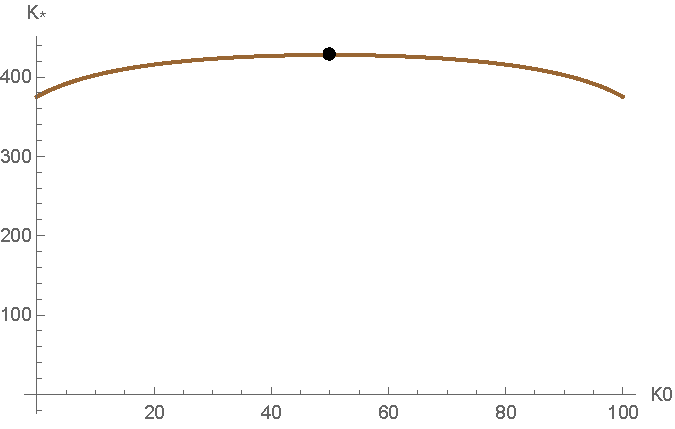
\includegraphics[width=0.45\textwidth]{Prob2_CapOpt/koptx_k0.pdf}
	\caption{Optimal capacity regarding the threshold value $x^*_C$ considering capacity levels $K_0 \in [0, 100)$ and its highest values at $\frac{1}{2 \alpha}=50$.}
	\label{fig:2_k0}
\end{figure}

On Figure \ref{fig:2_k1}, we obtain that $K^*_C$ increases with both drift and volatility, as it happened in the previous section. Note that again that, contrary to what happens for positive drift values, the growth of $K^*_C$ with $\mu$ is barely noticeable for negative values of $\mu$. FINANCIAL INTERPRETATION? This seems to be related again with the fact that for small drift values, the future expected demand value is smaller that for positive drift values. 
%Recall that the demand process evolves accordingly to a GBM and its expected value at time $t$ is given by $\mathds{E}^{X_0=x_0} [X_t]=x_0 e^{\mu t}$.

\begin{figure}[!htb]
	\begin{subfigmatrix}{2}
		\subfigure[$\mu \in ( -r,r )$ ]{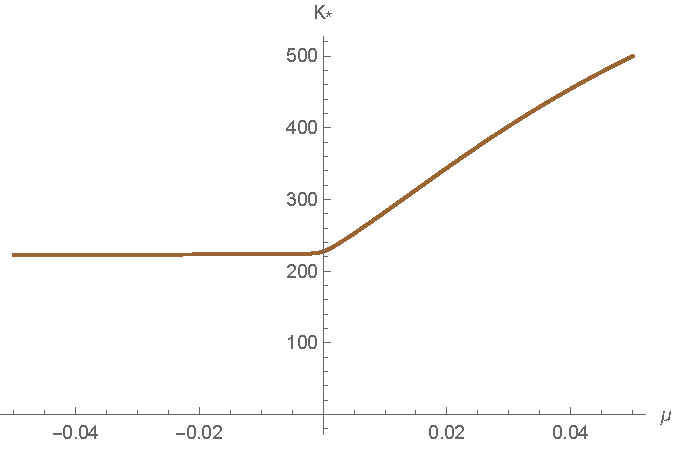
\includegraphics[width=0.45\textwidth]{Prob2_CapOpt/koptx_mu.pdf}}
		\subfigure[$\sigma \in (0,1)$]{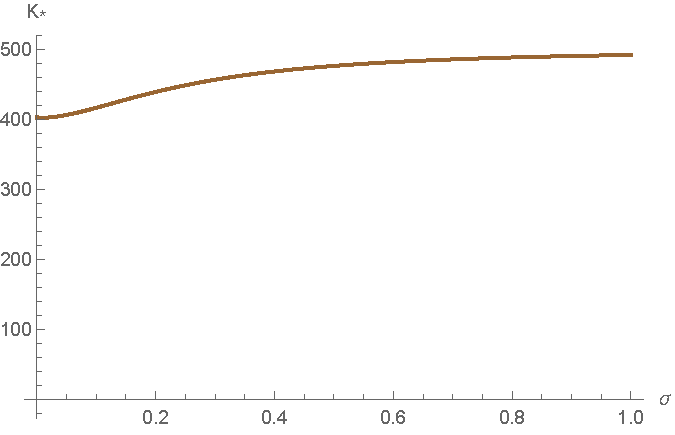
\includegraphics[width=0.45\textwidth]{Prob2_CapOpt/koptx_sigma.pdf}}
	\end{subfigmatrix}
	\caption{Optimal capacity regarding the threshold value $x^*_C$.}
	\label{fig:2_k1}
\end{figure}

Regarding innovation level $\theta$ and sensibility parameter $\delta$, we have on Figure \ref{fig:2_k3} that $K^*_C$ increases with them as well. Note that asymptotically, $K^*_C$ seems to increase linearly with $\theta$, as previously deduced.

\begin{figure}[!htb]
	\begin{subfigmatrix}{2}
		\subfigure[$ \theta \in ( 1, 10 )$]{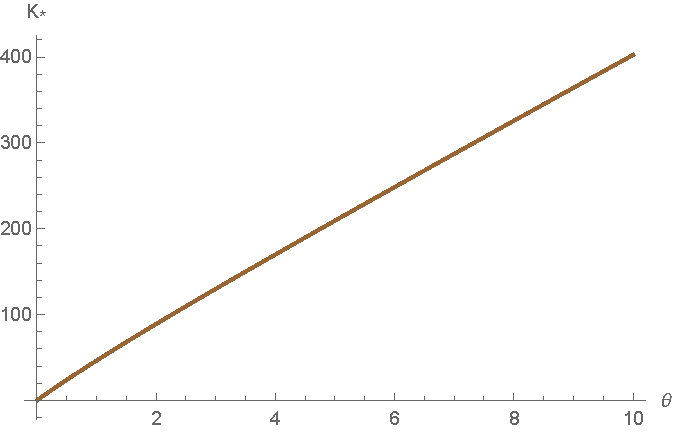
\includegraphics[width=0.45\textwidth]{Prob2_CapOpt/koptx_theta.pdf}}
		\subfigure[$ \delta \in (0,10)$]{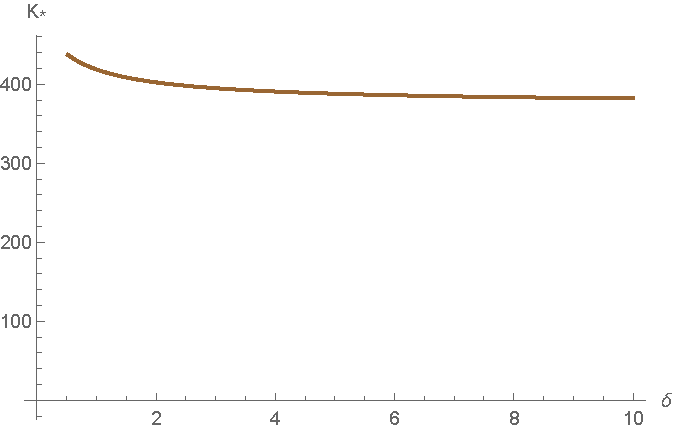
\includegraphics[width=0.45\textwidth]{Prob2_CapOpt/koptx_delta.pdf}}
	\end{subfigmatrix}
	\caption{Optimal capacity regarding the threshold value $x^*_C$.}
	\label{fig:2_k3}
\end{figure}

Regarding discount rate $r$ and sensibility parameter $\alpha$, we have on Figure \ref{fig:2_k2} that $K^*_C$ decreases with them, as expected.  

\begin{figure}[!htb]
	\begin{subfigmatrix}{2}
		\subfigure[$ r \in ( \mu, 1 )$]{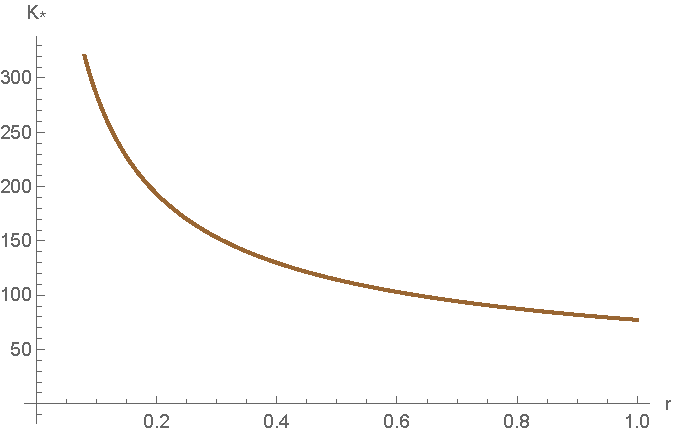
\includegraphics[width=0.45\textwidth]{Prob2_CapOpt/koptx_r.pdf}}
		\subfigure[$ \alpha \in (0,1)$]{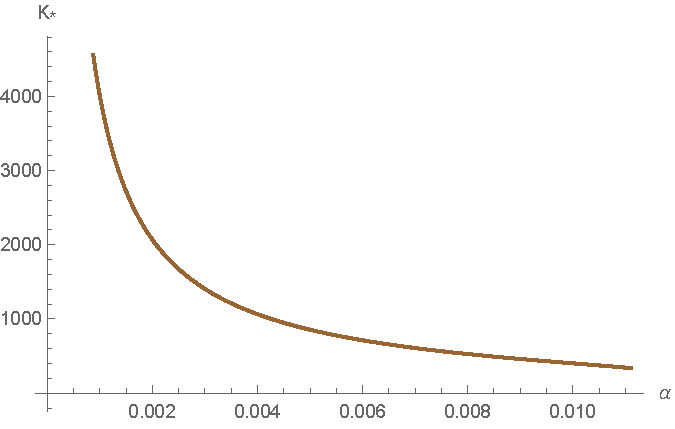
\includegraphics[width=0.45\textwidth]{Prob2_CapOpt/koptx_alpha.pdf}}
	\end{subfigmatrix}
	\caption{Optimal capacity regarding the threshold value $x^*_C$.}
	\label{fig:2_k2}
\end{figure}






















%%%%%%%%%%%%%%%%%%%%%%%%%%%%%%%%%%%%%%%%%%%%%%%%%%%%%%%%%%%%%%%%%%%%%%%%%

\pagebreak
%%%%%%%%%%%%%%%%%%%%%%%%%%%%%%%%%%%%%%%%%%%%%%%%%%%%%%%%%%%%%%%%%%%%%%%%
\section{Problem Description}
\label{section:problem}

Description of the baseline problem...


%%%%%%%%%%%%%%%%%%%%%%%%%%%%%%%%%%%%%%%%%%%%%%%%%%%%%%%%%%%%%%%%%%%%%%%%
\section{Baseline Solution}
\label{section:baseline}

Analysis of the baseline solution...


%%%%%%%%%%%%%%%%%%%%%%%%%%%%%%%%%%%%%%%%%%%%%%%%%%%%%%%%%%%%%%%%%%%%%%%%
\section{Enhanced Solution}
\label{section:enhanced}

Quest for the optimal solution...


% ----------------------------------------------------------------------
\subsection{Figures}
\label{subsection:figures}

Insert your section material and possibly a few figures...

Make sure all figures presented are referenced in the text!


% ----------------------------------------------------------------------
\subsubsection{Images}
\label{subsection:images}

\begin{figure}[!htb]
  \centering
  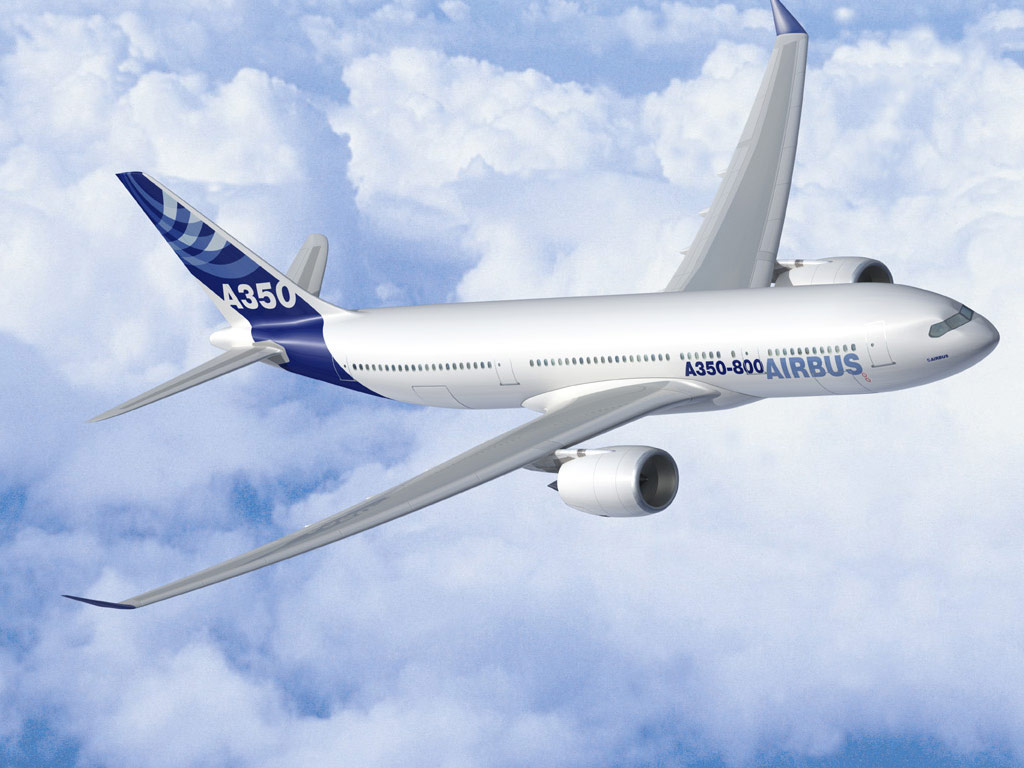
\includegraphics[width=0.25\textwidth]{Figures/Airbus_A350.jpg}
  \caption[Caption for figure in TOC.]{Caption for figure.}
  \label{fig:airbus1}
\end{figure}

\begin{figure}[!htb]
  \begin{subfigmatrix}{2}
    \subfigure[Airbus A320]{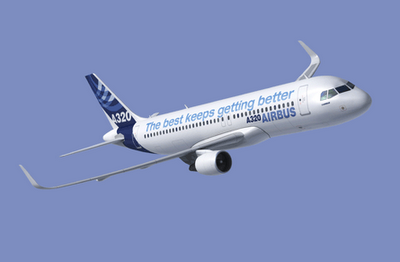
\includegraphics[width=0.49\linewidth]{Figures/Airbus_A320_sharklets.png}}
    \subfigure[Bombardier CRJ200]{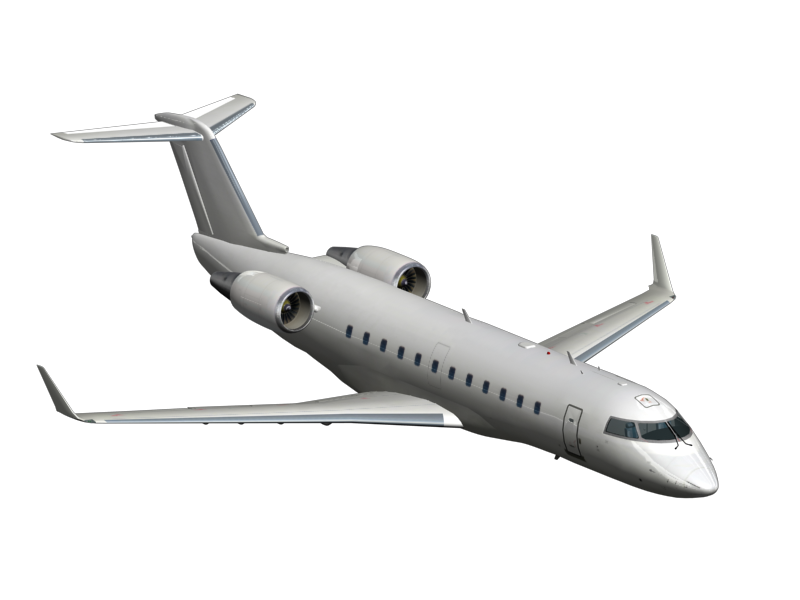
\includegraphics[width=0.49\linewidth]{Figures/Bombardier_CRJ200.png}}
  \end{subfigmatrix}
  \caption{Some aircrafts.}
  \label{fig:aircrafts}
\end{figure}

Make reference to Figures \ref{fig:airbus1} and \ref{fig:aircrafts}.

By default, the supported file types are {\it .png,.pdf,.jpg,.mps,.jpeg,.PNG,.PDF,.JPG,.JPEG}.

See \url{http://mactex-wiki.tug.org/wiki/index.php/Graphics_inclusion} for adding support to other extensions.


% ----------------------------------------------------------------------
\subsubsection{Drawings}
\label{subsection:drawings}

Insert your subsection material and for instance a few drawings...

The schematic illustrated in Fig.~\ref{fig:algorithm} can represent some sort of algorithm.

\begin{figure}[!htb]
  \centering
  \scriptsize
%  \footnotesize 
%  \small
  \setlength{\unitlength}{0.9cm}
  \begin{picture}(8.5,6)
    \linethickness{0.3mm}

    \put(3,6){\vector(0,-1){1}}
    \put(3.5,5.4){$\bf \alpha$}
    \put(3,4.5){\oval(6,1){}}
    %\put(0,4){\framebox(6,1){}}
    \put(0.3,4.4){Grid Generation: \quad ${\bf x} = {\bf x}\left({\bf \alpha}\right)$}

    \put(3,4){\vector(0,-1){1}}
    \put(3.5,3.4){$\bf x$}
    \put(3,2.5){\oval(6,1){}}
    %\put(0,2){\framebox(6,1){}}
    \put(0.3,2.4){Flow Solver: \quad ${\cal R}\left({\bf x},{\bf q}\left({\bf x}\right)\right) = 0$}

    \put(6.0,2.5){\vector(1,0){1}}
    \put(6.4,3){$Y_1$}

    \put(3,2){\vector(0,-1){1}}
    \put(3.5,1.4){$\bf q$}
    \put(3,0.5){\oval(6,1){}}
    %\put(0,0){\framebox(6,1){}}
    \put(0.3,0.4){Structural Solver: \quad ${\cal M}\left({\bf x},{\bf q}\left({\bf x}\right)\right) = 0$}

    \put(6.0,0.5){\vector(1,0){1}}
    \put(6.4,1){$Y_2$}

    %\put(7.8,2.5){\oval(1.6,5){}}
    \put(7.0,0){\framebox(1.6,5){}}
    \put(7.1,2.5){Optimizer}
    \put(7.8,5){\line(0,1){1}}
    \put(7.8,6){\line(-1,0){4.8}}
  \end{picture}
  \caption{Schematic of some algorithm.}
  \label{fig:algorithm}
\end{figure}


% ----------------------------------------------------------------------
\subsection{Equations}
\label{subsection:equations}

Equations can be inserted in different ways.

The simplest way is in a separate line like this

\begin{equation}
  \frac{{\rm d} q_{ijk}}{{\rm d} t} + {\cal R}_{ijk}({\bf q}) = 0 \,.
\label{eq:ode}
\end{equation}

If the equation is to be embedded in the text. One can do it like this ${\partial {\cal R}}/{\partial {\bf q}}=0$.

It may also be split in different lines like this

\begin{eqnarray}
  {\rm Minimize}   && Y({\bf \alpha},{\bf q}({\bf \alpha}))            \nonumber           \\
  {\rm w.r.t.}     && {\bf \alpha} \,,                                 \label{eq:minimize} \\
  {\rm subject~to} && {\cal R}({\bf \alpha},{\bf q}({\bf \alpha})) = 0 \nonumber           \\
                   &&       C ({\bf \alpha},{\bf q}({\bf \alpha})) = 0 \,. \nonumber
\end{eqnarray}

It is also possible to use subequations. Equations~\ref{eq:continuity}, \ref{eq:momentum} and \ref{eq:energy} form the Naver--Stokes equations~\ref{eq:NavierStokes}.

\begin{subequations}
    \begin{equation}
    \frac{\partial \rho}{\partial t} + \frac{\partial}{\partial x_j}\left( \rho u_j \right) = 0 \,,
    \label{eq:continuity}
    \end{equation}
    \begin{equation}
    \frac{\partial}{\partial t}\left( \rho u_i \right) + \frac{\partial}{\partial x_j} \left( \rho u_i u_j + p \delta_{ij} - \tau_{ji} \right) = 0, \quad i=1,2,3 \,,
    \label{eq:momentum}
    \end{equation}
    \begin{equation}
        \frac{\partial}{\partial t}\left( \rho E \right) + \frac{\partial}{\partial x_j} \left( \rho E u_j + p u_j - u_i \tau_{ij} + q_j \right) = 0 \,.
    \label{eq:energy}
    \end{equation}
\label{eq:NavierStokes}%
\end{subequations}


% ----------------------------------------------------------------------
\subsection{Tables}
\label{section:tables}

Insert your subsection material and for instance a few tables...

Make sure all tables presented are referenced in the text!

Follow some guidelines when making tables:

\begin{itemize}
  \item Avoid vertical lines
  \item Avoid “boxing up” cells, usually 3 horizontal lines are enough: above, below, and after heading
  \item Avoid double horizontal lines
  \item Add enough space between rows
\end{itemize}

\begin{table}[!htb]
  \renewcommand{\arraystretch}{1.2} % more space between rows
  \centering
  \begin{tabular}{lccc}
    \toprule
    Model           & $C_L$ & $C_D$ & $C_{M y}$ \\
    \midrule
    Euler           & 0.083 & 0.021 & -0.110    \\
    Navier--Stokes  & 0.078 & 0.023 & -0.101    \\
    \bottomrule
  \end{tabular}
  \caption[Table caption shown in TOC.]{Table caption.}
  \label{tab:aeroCoeff}
\end{table}

Make reference to Table \ref{tab:aeroCoeff}.

Tables \ref{tab:memory} and \ref{tab:multipleColumns} are examples of tables with merging columns:

\begin{table}[!htb]
  \renewcommand{\arraystretch}{1.2} % more space between rows
  \centering
  \begin{tabular}[]{lrr}
    \toprule
                & \multicolumn{2}{c}{\underline{Virtual memory [MB]}} \\
                & Euler       & Navier--Stokes \\
    \midrule
      Wing only &  1,000      &    2,000       \\
      Aircraft  &  5,000      &   10,000       \\
      (ratio)   & $5.0\times$ & $5.0\times$    \\
    \bottomrule
  \end{tabular}
  \caption{Memory usage comparison (in MB).}
  \label{tab:memory}
\end{table}

\begin{table}[!htb]
  \centering
  \renewcommand{\arraystretch}{1.2} % more space between rows
  \begin{tabular}{@{}rrrrcrrr@{}} % remove space to the vertical edges @{}...@{}
    \toprule
      & \multicolumn{3}{c}{$w = 2$} & \phantom{abc} & \multicolumn{3}{c}{$w = 4$} \\
    \cmidrule{2-4}
    \cmidrule{6-8}
      & $t=0$ & $t=1$ & $t=2$ && $t=0$ & $t=1$ & $t=2$ \\
    \midrule
      $dir=1$
      \\
      $c$ &  0.07 &  0.16 &  0.29 &&  0.36 &  0.71 &   3.18 \\
      $c$ & -0.86 & 50.04 &  5.93 && -9.07 & 29.09 &  46.21 \\
      $c$ & 14.27 &-50.96 &-14.27 && 12.22 &-63.54 &-381.09 \\
      $dir=0$
      \\
      $c$ &  0.03 &  1.24 &  0.21 &&  0.35 & -0.27 &  2.14 \\
      $c$ &-17.90 &-37.11 &  8.85 &&-30.73 & -9.59 & -3.00 \\
      $c$ &105.55 & 23.11 &-94.73 &&100.24 & 41.27 &-25.73 \\
    \bottomrule
  \end{tabular}
  \caption{Another table caption.}
  \label{tab:multipleColumns}
\end{table}

An example with merging rows can be seen in Tab.\ref{tab:multipleRows}.

\begin{table}[!htb]
  \renewcommand{\arraystretch}{1.2} % more space between rows
  \centering
  \begin{tabular}{ccccc}
    \toprule
      \multirow{2}{*}{ABC} & \multicolumn{4}{c}{header} \\
      \cmidrule{2-5} & 1.1 & 2.2 & 3.3 & 4.4 \\
    \midrule
      \multirow{2}{*}{IJK} & \multicolumn{2}{c}{\multirow{2}{*}{group}} & 0.5 & 0.6 \\
      \cmidrule{4-5}       & \multicolumn{2}{c}{}                       & 0.7 & 1.2 \\
    \bottomrule
  \end{tabular}
  \caption{Yet another table caption.}
  \label{tab:multipleRows}
\end{table}

If the table has too many columns, it can be scaled to fit the text widht, as in Tab.\ref{tab:scale}.
\begin{table}[!htb]
  \renewcommand{\arraystretch}{1.2} % more space between rows
  \centering
  \resizebox*{\textwidth}{!}{%
    \begin{tabular}[]{lcccccccccc}
      \toprule
        Variable &  a  &  b  &  c  &  d  &  e  &  f  &  g  &  h  &  i  &  j  \\
      \midrule
        Test 1   &  10,000 &  20,000 &  30,000 &  40,000 &  50,000 &  60,000 &  70,000 &  80,000 &  90,000 & 100,000 \\
        Test 2   &  20,000 &  40,000 &  60,000 &  80,000 & 100,000 & 120,000 & 140,000 & 160,000 & 180,000 & 200,000 \\
      \bottomrule
    \end{tabular}
  }%
  \caption{Very wide table.}
  \label{tab:scale}%
\end{table}


% ----------------------------------------------------------------------
\subsection{Mixing}
\label{section:mixing}

If necessary, a figure and a table can be put side-by-side as in Fig.\ref{fig:side_by_side}

\begin{figure}[!htb]
  \begin{minipage}[b]{0.60\linewidth}
    \centering
    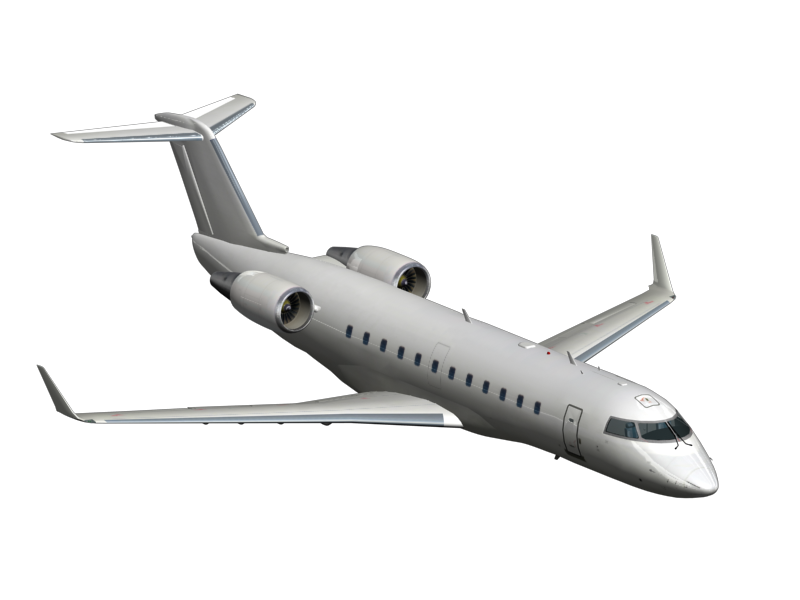
\includegraphics[width=\linewidth]{Figures/Bombardier_CRJ200}
  \end{minipage}%
  \begin{minipage}[b]{0.30\linewidth}
    \centering
    \begin{tabular}[b]{lll}
      \toprule
        \multicolumn{3}{c}{Legend} \\
      \midrule
        A & B & C \\
        0 & 0 & 0 \\
        0 & 1 & 0 \\
        1 & 0 & 0 \\
        1 & 1 & 1 \\
      \bottomrule
    \end{tabular}
    \vspace{5em}
  \end{minipage}
\caption{Figure and table side-by-side.}
\label{fig:side_by_side}
\end{figure}

